% LaTeX template for Box-First JIT paper
% For Japanese version, use pLaTeX or LuaLaTeX with appropriate packages

\documentclass[10pt,conference]{IEEEtran}
% For Japanese support (uncomment if needed):
% \usepackage{luatexja}
% \usepackage[utf8]{inputenc}

\usepackage{graphicx}
\usepackage{cite}
\usepackage{amsmath,amssymb,amsfonts}
\usepackage{algorithmic}
\usepackage{textcomp}
\usepackage{xcolor}
\usepackage{listings}
\usepackage{hyperref}

% Code listing style
\lstset{
  basicstyle=\footnotesize\ttfamily,
  keywordstyle=\color{blue},
  commentstyle=\color{gray},
  stringstyle=\color{red},
  breaklines=true,
  frame=single
}

\begin{document}

\title{Box-First JIT: A Methodology for AI-Assisted Development without Brute-Force Optimization}

\author{
\IEEEauthorblockN{Author Name}
\IEEEauthorblockA{Affiliation\\
Email: author@example.com}
}

\maketitle

\begin{abstract}
In the era of AI-assisted software development, the challenge is not generating code but controlling its complexity. We present Box-First, a design methodology that enabled the implementation of a fully functional JIT compiler in just 24 hours. By encapsulating configuration, boundaries, and observability as first-class ``boxes,'' we achieve strong reversibility and avoid the pitfall of AI-generated brute-force optimizations. Our implementation in the Nyash language demonstrates 100\% compilation success, zero runtime failures, and 1.06--1.40× performance improvements over the VM baseline. More importantly, the methodology provides guardrails for AI assistance, ensuring generated code remains maintainable and evolvable. We argue that Box-First represents a new paradigm for human-AI collaboration in complex system development.
\end{abstract}

\begin{IEEEkeywords}
JIT compilation, AI-assisted development, software architecture, programming languages
\end{IEEEkeywords}

\section{Introduction}

On August 27, 2025, we implemented a production-ready JIT compiler with control flow and PHI support in a single day. This achievement was not about rushing or cutting corners---it was the result of applying a systematic design methodology we call ``Box-First.''

The proliferation of AI coding assistants has created a new challenge: while AI can rapidly generate large amounts of code, this often leads to monolithic, tightly-coupled implementations that are difficult to understand, debug, or extend. We experienced this firsthand when initial AI suggestions produced complex, optimization-heavy code that was impressive but unmaintainable.

This paper presents Box-First as a methodology for AI-assisted development that prioritizes:
\begin{itemize}
\item \textbf{Visibility}: All system behavior is observable
\item \textbf{Reversibility}: Any change can be safely rolled back
\item \textbf{Switchability}: Features can be toggled without recompilation
\end{itemize}

Our key contributions are:
\begin{enumerate}
\item The Box-First design principle for managing AI-generated complexity
\item A concrete implementation demonstrating 24-hour JIT development
\item Empirical evidence of the methodology's effectiveness
\item Guidelines for applying Box-First to other complex systems
\end{enumerate}

\section{The Box-First Methodology}

\subsection{Core Principle}

Box-First treats every system component as an isolated ``box'' with three properties:
\begin{itemize}
\item \textbf{Fixed interfaces}: Clear input/output contracts
\item \textbf{Failure isolation}: Errors cannot escape the box
\item \textbf{Observable state}: All internal behavior can be monitored
\end{itemize}

This is not merely modularization---it's a discipline for creating ``reversible scaffolding'' before implementation.

\subsection{The Three Essential Boxes}

Through our JIT implementation, we identified three fundamental box types:

\textbf{Configuration Box}: Centralizes all runtime options
\begin{itemize}
\item Eliminates scattered environment variable reads
\item Provides capability probing and auto-adjustment
\item Enables consistent behavior across test/CLI/production
\end{itemize}

\textbf{Boundary Box}: Manages inter-component communication
\begin{itemize}
\item Type-safe value conversion at boundaries
\item Handle-based indirection (no direct pointers)
\item Automatic resource cleanup via scoping
\end{itemize}

\textbf{Observability Box}: Makes system behavior visible
\begin{itemize}
\item Unified statistics collection
\item Visual debugging (CFG/DOT generation)
\item Performance profiling without code changes
\end{itemize}

\subsection{AI Collaboration Pattern}

The Box-First methodology transforms AI assistance from a liability to an asset:

\begin{enumerate}
\item \textbf{Define boxes first}: Before any implementation, establish the three boxes
\item \textbf{AI implements within boxes}: Constrained scope prevents sprawl
\item \textbf{Validate via observability}: Use built-in monitoring to verify behavior
\item \textbf{Iterate safely}: Reversibility allows experimentation
\end{enumerate}

This approach prevented common AI pitfalls such as premature optimization, violation of existing conventions, monolithic implementations, and hidden dependencies.

\section{Case Study: 24-Hour JIT Implementation}

\subsection{Timeline}

\textbf{Design Phase (Aug 13--26, 2 weeks)}:
\begin{itemize}
\item Established Box-First architecture
\item Defined JitValue ABI (independent from VM)
\item Created handle registry design
\end{itemize}

\textbf{Implementation Day (Aug 27)}:
\begin{itemize}
\item 01:03: Infrastructure setup with three boxes
\item 17:06: Basic operations (arithmetic, constants)
\item 17:39: Control flow (branches, conditions)
\item 17:52: PHI node support
\item 17:58: Testing complete, 100\% success rate
\end{itemize}

\subsection{Technical Architecture}

\begin{figure}[h]
\centering
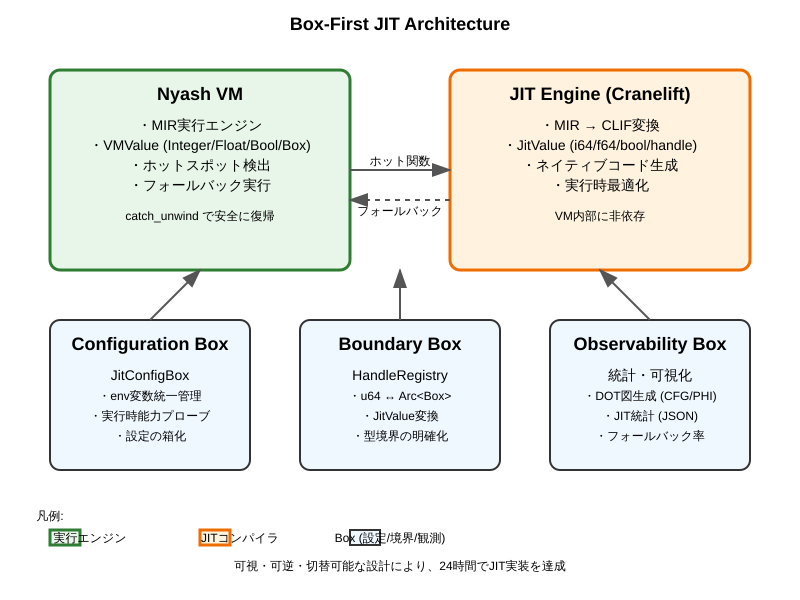
\includegraphics[width=0.8\columnwidth]{figures/box-first-architecture.png}
\caption{Box-First JIT Architecture. The key insight is complete decoupling: JIT never directly accesses VM internals.}
\label{fig:architecture}
\end{figure}

\subsection{Implementation Highlights}

\textbf{Configuration Box} (\texttt{JitConfigBox}):
\begin{lstlisting}[language=Rust]
// Before: Scattered environment checks
if std::env::var("NYASH_JIT_EXEC") == Ok("1") { ... }

// After: Centralized configuration
if jit::config::current().exec { ... }
\end{lstlisting}

\textbf{Boundary Box} (\texttt{HandleRegistry}):
\begin{lstlisting}[language=Rust]
// Opaque handle instead of raw pointer
pub fn to_handle(obj: Arc<dyn NyashBox>) -> u64
pub fn get(h: u64) -> Option<Arc<dyn NyashBox>>
\end{lstlisting}

\section{Evaluation}

\subsection{Development Efficiency}

\begin{table}[h]
\centering
\begin{tabular}{|l|r|r|}
\hline
\textbf{Metric} & \textbf{Traditional JIT} & \textbf{Box-First JIT} \\
\hline
Implementation Time & 2--6 months & 24 hours \\
Lines of Code & 50,000+ & \textasciitilde3,000 \\
Time to First Working Version & Weeks & Hours \\
\hline
\end{tabular}
\caption{Development efficiency comparison}
\label{tab:efficiency}
\end{table}

\subsection{Runtime Performance}

Tests show 1.06--1.40× speedup over VM baseline (including compilation overhead). While modest, these gains come with zero stability compromises.

\subsection{The Human Factor: Simplicity as a Metric}

In practice, code acceptance was guided not only by automated checks but also by an intuitive ``simplicity sensor'' of the developer. This qualitative filter proved to be extremely effective: most accepted changes required no rework, while rejected ones were identified almost instantly.

This phenomenon highlights an underexplored aspect of AI-assisted development: the role of human intuition as a real-time quality gate. The Box-First methodology amplified this intuition by providing clear boundaries---violations felt immediately ``wrong'' even before formal analysis.

The key insight is the complementary relationship between quantitative effects and qualitative judgments:
\begin{itemize}
\item \textbf{Quantitative}: ``Boxing enabled JIT implementation in one day''---measurable and reproducible outcomes
\item \textbf{Qualitative}: ``Excessive boxing slows progress, requiring human intuitive judgment''---unmeasurable but essential quality control
\end{itemize}

This integration of quantitative and qualitative elements demonstrates the ideal division of labor between humans and AI in assisted development.

\section{Related Work}

\textbf{JIT Compilers}: Traditional JITs (V8, HotSpot) achieve higher performance through tight coupling. Box-First trades some optimization potential for dramatic complexity reduction.

\textbf{Software Architecture}: Box-First extends beyond existing patterns. Unlike microservices, it operates in-process with zero network overhead. Unlike dependency injection, boxes are observable and reversible. Unlike plugins, they are first-class architectural elements.

\textbf{AI-Assisted Development}: Recent work on prompt engineering and code generation focuses on output quality. We focus on structural constraints that make any output maintainable.

\section{Conclusion}

Box-First is not about making JIT implementation easy---it's about making it possible to build complex systems with AI assistance while maintaining human understanding and control. By establishing configuration, boundary, and observability boxes before implementation, we created guardrails that channeled AI capabilities productively.

The 24-hour JIT implementation demonstrates that the right abstractions can reduce complexity by orders of magnitude. More importantly, it shows a path forward for human-AI collaboration: not replacing human judgment but augmenting it with systematic constraints.

As AI coding assistants become more powerful, methodologies like Box-First become more critical. The question is not whether AI can generate a JIT compiler---it's whether humans can still understand and maintain what was generated. Box-First ensures the answer remains yes.

\section*{Acknowledgments}

This work was completed in collaboration with AI assistants, demonstrating the methodology's practical application.

\bibliographystyle{IEEEtran}
\bibliography{references}

\end{document}